%--------------------------------------------------
% Estudo de caso MDA
%--------------------------------------------------

\documentclass[11pt]{article}

% Configurações

\usepackage[utf8]{inputenc}
\usepackage{geometry}
\usepackage{graphicx}

\geometry{a4paper}

\usepackage{booktabs}
\usepackage{array}
\usepackage{paralist}
\usepackage{verbatim}
\usepackage{subfig}
\usepackage{color}
\usepackage{listings}
\usepackage{fancyhdr}
\pagestyle{fancy}
\renewcommand{\headrulewidth}{0pt}
\lhead{}\chead{}\rhead{}
\lfoot{}\cfoot{\thepage}\rfoot{}

\usepackage{sectsty}
\allsectionsfont{\sffamily\mdseries\upshape}

\usepackage[nottoc,notlof,notlot]{tocbibind}
\usepackage[titles,subfigure]{tocloft}
\renewcommand{\cftsecfont}{\rmfamily\mdseries\upshape}
\renewcommand{\cftsecpagefont}{\rmfamily\mdseries\upshape}

\usepackage{graphicx}
\usepackage{pdflscape}
\usepackage{caption}

\captionsetup[lstlisting]{font={small,tt}}

\lstset{ %
language=Java,                % choose the language of the code
basicstyle=\footnotesize,       % the size of the fonts that are used for the code
numbers=left,                   % where to put the line-numbers
numberstyle=\footnotesize,      % the size of the fonts that are used for the line-numbers
stepnumber=1,                   % the step between two line-numbers. If it is 1 each line will be numbered
numbersep=5pt,                  % how far the line-numbers are from the code
backgroundcolor=\color{white},  % choose the background color. You must add \usepackage{color}
showspaces=false,               % show spaces adding particular underscores
showstringspaces=false,         % underline spaces within strings
showtabs=false,                 % show tabs within strings adding particular underscores
frame=single,           % adds a frame around the code
tabsize=4,          % sets default tabsize to 2 spaces
captionpos=b,           % sets the caption-position to bottom
breaklines=true,        % sets automatic line breaking
breakatwhitespace=false,    % sets if automatic breaks should only happen at whitespace
escapeinside={\%*}{*)}          % if you want to add a comment within your code
}

\lstset{frameround=fttt}

% Fim das configurações
% Início do documento

\title{Pizzaria Geek: Um estudo MDA}
\author{Paulo Ortolan \and André Nucci \and Paulo Fernandes}

\begin{document}
\maketitle

\section{Descrição do Projeto}

A pizzaria Geek, famosa por abrigar nerds, geeks e fãs de RPGs como Dungeons \& Dragons e GURPS, quer melhorar seu sistema, criado em uma feira medieval no verão de 87 (a.k.a. Clipper 87) para algo mais moderno como o sistema LCARS da Nova Geração da Enterprise.

No entanto, o mestre dos magos da pizzaria é cético quanto à essa modernização. Ele não acha que um sistema pode ser feito como armaduras do Iron Man. Sua crença se resume à frases de efeitos do Sr. Miyagi e conselhos inversos do Yoda (Anos 80 isso é Hmmmmm!). Ele quer ser convencido que suas pizzas mais saborosas, como a Obi Wan Calzone ou Ham Solo, vão ser vendidas melhor com o novo sistema.

Este relatório tem como objetivo mostrar que isso é possível e não está sob domínio exclusivo de onerosos estúdios de Hollywood ou fazem parte do imaginário da Ficção Científica.

\section{Diagrama de Classes}

Nesta seção, seguem os diagramas de classes gerados pela ferramenta Modelio.

\begin{figure}[h!]
 \centering
 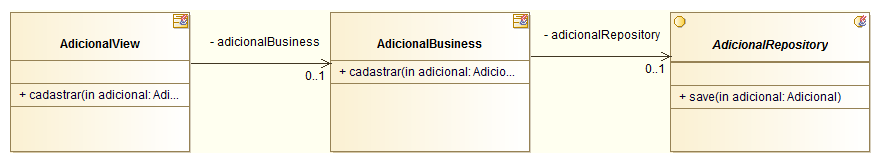
\includegraphics[scale=0.5]{capitulo02/diagramaClassesCadastrarAdicionais.png}
 \caption{Diagrama de Classes Cadastrar Adicionais}
\end{figure}

\begin{figure}[h!]
 \centering
 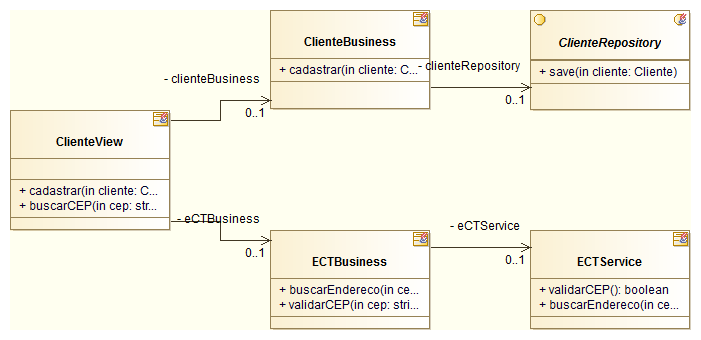
\includegraphics[scale=0.5]{capitulo02/diagramaClassesCadastrarClientes.png}
 \caption{Diagrama de Classes Cadastrar Adicionais}
\end{figure}

\begin{figure}[h!]
 \centering
 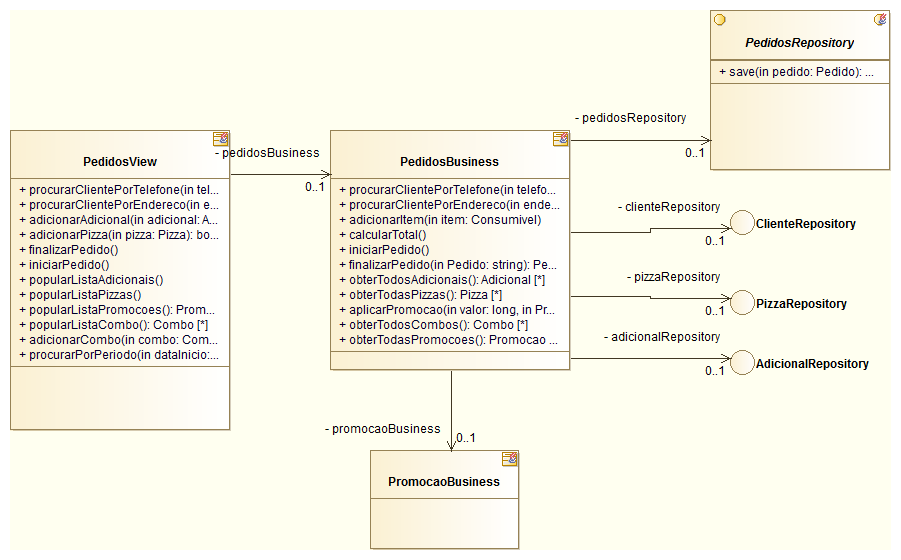
\includegraphics[scale=0.5]{capitulo02/diagramaClassesCadastrarPedidos.png}
 \caption{Diagrama de Classes Cadastrar Pedidos}
\end{figure}

\begin{figure}[h!]
 \centering
 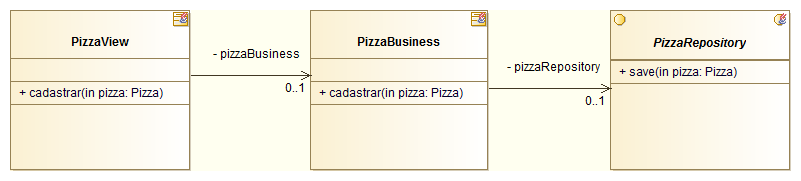
\includegraphics[scale=0.5]{capitulo02/diagramaClassesCadastrarPizzas.png}
 \caption{Diagrama de Classes Cadastrar Pizzas}
\end{figure}

\begin{figure}[h!]
 \centering
 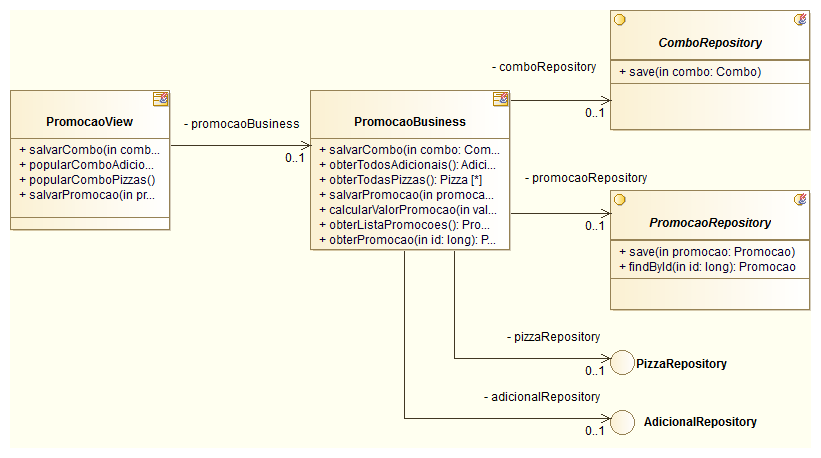
\includegraphics[scale=0.5]{capitulo02/diagramaClassesCadastrarPromocoes.png}
 \caption{Diagrama de Classes Cadastrar Promoções}
\end{figure}

\begin{figure}[h!]
 \centering
 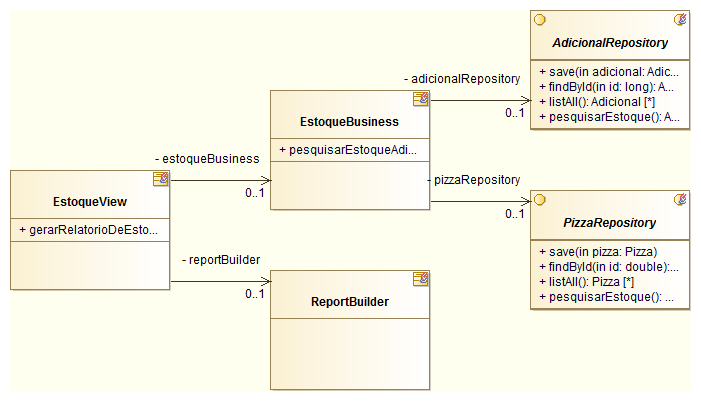
\includegraphics[scale=0.5]{capitulo02/diagramaClassesEmitirRelatorioEstoque.png}
 \caption{Diagrama de Classes Emitir Relatório de Estoque}
\end{figure}

\begin{figure}[h!]
 \centering
 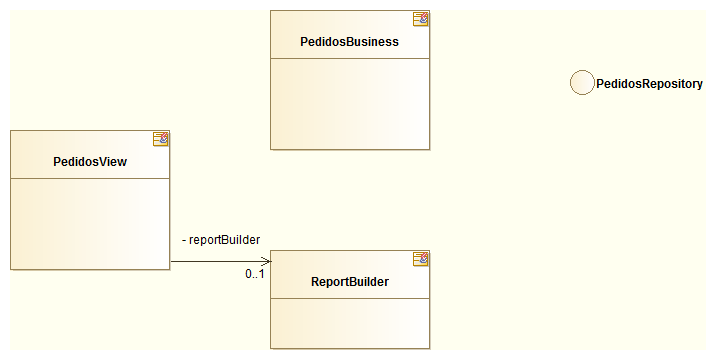
\includegraphics[scale=0.5]{capitulo02/diagramaClassesEmitirRelatorioPedido.png}
 \caption{Diagrama de Classes Emitir Relatório de Pedido}
\end{figure}

\begin{figure}[h!]
 \centering
 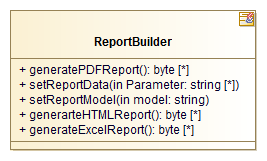
\includegraphics[scale=0.5]{capitulo02/diagramaClassesReportBuilder.png}
 \caption{Diagrama de Classes Report Builder}
\end{figure}

\begin{landscape}
\begin{figure}[h!]
 \centering
 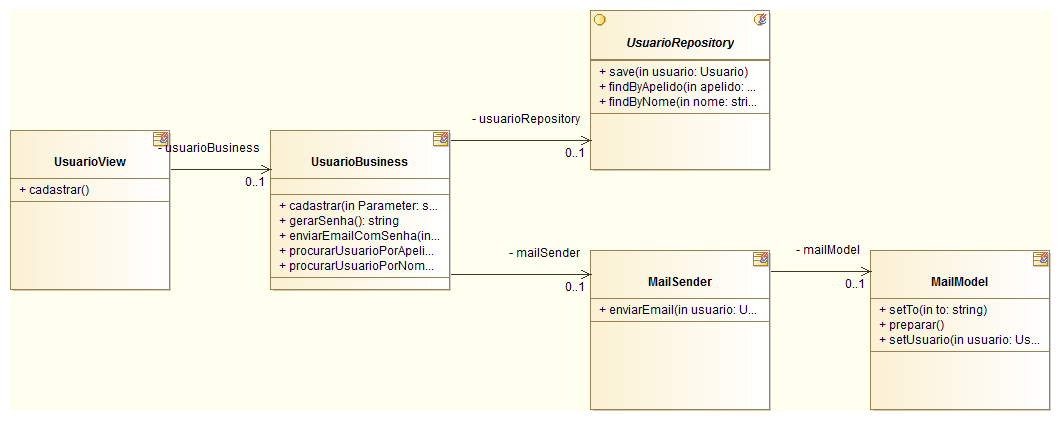
\includegraphics[scale=0.5]{capitulo02/diagramaClassesCadastrarUsuarios.png}
 \caption{Diagrama de Classes Cadastrar Usuários}
\end{figure}
\end{landscape}

\begin{landscape}
\begin{figure}[h!]
 \centering
 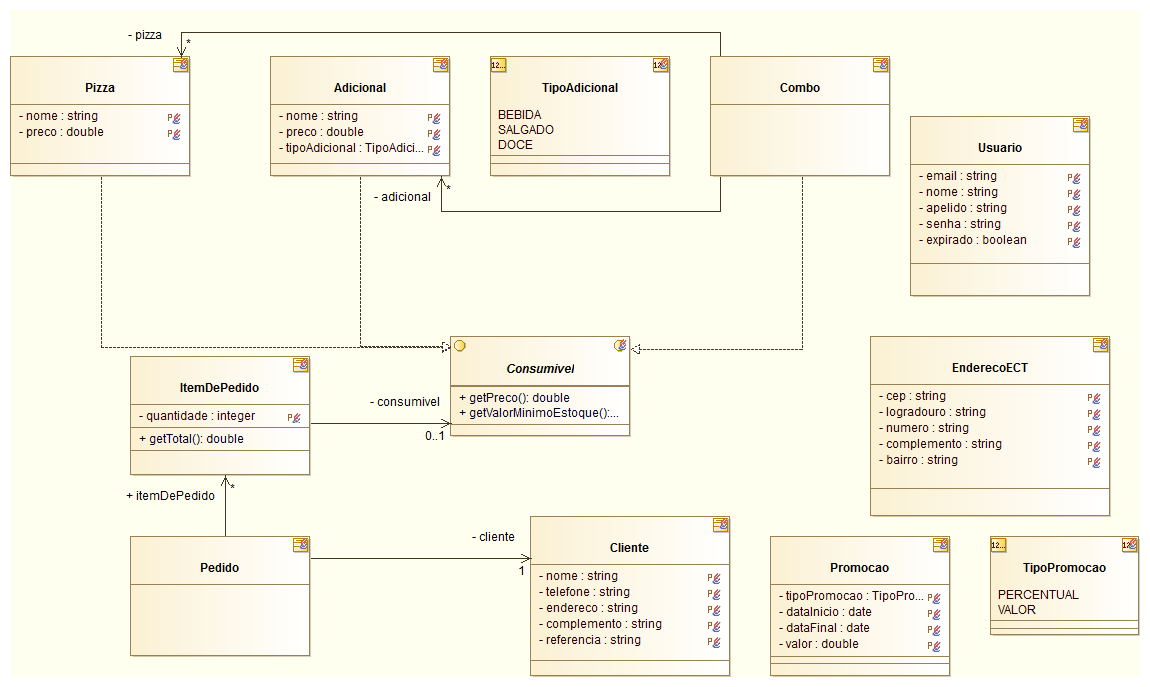
\includegraphics[scale=0.5]{capitulo02/diagramaClassesMER.png}
 \caption{Diagrama de Classes Modelo Entidade Relacionamento}
\end{figure}
\end{landscape}


\section{Reflexão Transformação}

	Nesta seção segue a reflexão inicial.

\subsection{Avaliação do código gerado}

	O código foi gerado conforme o modelo. Nota-se a existência de algumas anotações da ferramenta o que prejudica um pouco a leitura do código. Para os tipos múltiplos, a ferramenta gera um tipo List parametrizado pelo tipo em questão. A ferramenta gera um método getter privado para uma propriedade privada (configuração, falta inibição?).

\subsection{Utilidade prática desta ferramenta}

	A utilidade prática é de aumentar a produtividade com a geração automática do código através da diagramação.

\subsection{Elementos faltantes}

\begin{tabular}{| p{5cm} | p{4cm} | p{5cm} |}
  \hline
  \textbf{Elemento(s)} & \textbf{Diagrama(s) UML Correspondente(s)} & \textbf{Grau de Dificuldade de Transformação Automática} \\
	\hline
  Sequencia mínima de interação entre as classes & Diagrama de Sequência & ? \\
	\hline
  Definição da plataforma específica & &  \\
	\hline
  Importação de bibliotecas estrangeiras & Diagrama de Componentes & ? \\
	\hline
  Definição de Pacotes & Diagrama de Classes & ? \\
	\hline
\end{tabular}

\section{Código gerado}

Nesta seção segue a listagem do código gerado pela ferramenta Modelio.
\newline

\lstinputlisting[language=Java, caption=Bean Classe Adicional]{capitulo04/Adicional.java}

\section{Código Sintaxe PL/0}

Nesta seção segue a listagem do código sintático em Java para a linguagem PL/0.
\newline

\lstinputlisting[language=Java, caption=Classe Java para análise sintática da linguagem PL/0]{capitulo05/Sintatico.java}

\section{Código de uma classe Java}

Listagem da calsse PedidosBusiness.java.
\newline

\lstinputlisting[language=Java, caption=Implementação padrão da classe PedidosBusiness]{capitulo06/PedidosBusiness.java}

\section{Diagramas Adicionais do Projeto}

%\includegraphics{tex.jpg}

\section{Mapeamento}

ASDF.

\section{Autômato Sintático Classes Java}

Nesta seção segue o código sintático Java.

% ---------------------------
\subsection{JavaClass}

\begin{lstlisting}
JavaClass

    packageDefinition
    importsDefinition
    classBody
\end{lstlisting}

\begin{figure}[h!]
 \centering
 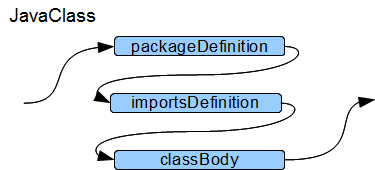
\includegraphics{capitulo09/JavaClass.png}
 \caption{Classe Java}
\end{figure}
% ---------------------------
\subsection{packageDefinition}

\begin{lstlisting}
packageDefinition

   package pathToClass ;
\end{lstlisting}

\begin{figure}[h!]
 \centering
 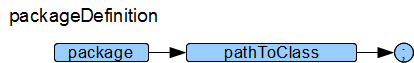
\includegraphics{capitulo09/packageDefinition.png}
 \caption{Definição de pacote}
\end{figure}
% ---------------------------
\subsection{pathToClass}

\begin{lstlisting}
pathToClass

   pathIdentifier
   pathIdentifier . 
\end{lstlisting}

\begin{figure}[h!]
 \centering
 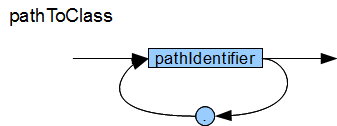
\includegraphics{capitulo09/pathToClass.png}
 \caption{Caminho da classe}
\end{figure}
% ---------------------------
\subsection{pathIdentifier}

\begin{lstlisting}
pathIdentifier

   [a-z]
	
\end{lstlisting}

\begin{figure}[h!]
 \centering
 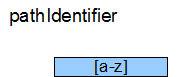
\includegraphics{capitulo09/pathIdentifier.png}
 \caption{Identificador de caminho}
\end{figure}
% ---------------------------
\subsection{importsDefinition}

\begin{lstlisting}
importsDefinition

   import canonicalName ;

\end{lstlisting}

\begin{figure}[h!]
 \centering
 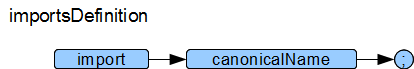
\includegraphics{capitulo09/importsDefinition.png}
 \caption{Definição de import}
\end{figure}
% ---------------------------
\subsection{canonicalName}

\begin{lstlisting}
canonicalName

   pathToClass . ClassName

\end{lstlisting}

\begin{figure}[h!]
 \centering
 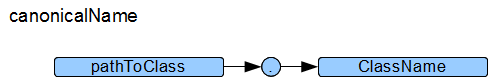
\includegraphics{capitulo09/canonicalName.png}
 \caption{Nome canônico da classe}
\end{figure}
% ---------------------------
\subsection{ClassName}

\begin{lstlisting}
ClassName

   ([A-Z][a-z0-9]+){2,}

\end{lstlisting}

\begin{figure}[h!]
 \centering
 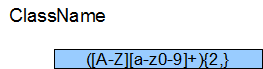
\includegraphics{capitulo09/ClassName.png}
 \caption{Nome da classe}
\end{figure}
% ---------------------------
\subsection{classBody}

\begin{lstlisting}
classBody

   public class ClassName { members }

\end{lstlisting}

\begin{figure}[h!]
 \centering
 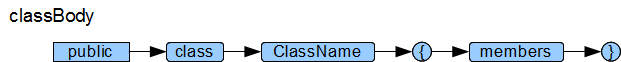
\includegraphics{capitulo09/classBody.png}
 \caption{Declaração de corpo da classe}
\end{figure}
% ---------------------------
\subsection{members}

\begin{lstlisting}
members

   []
   attribute
   method

\end{lstlisting}

\begin{figure}[h!]
 \centering
 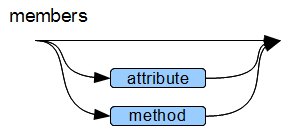
\includegraphics{capitulo09/members.png}
 \caption{Membros da classe}
\end{figure}
% ---------------------------
\subsection{attribute}

\begin{lstlisting}
attribute

   accessor modifier variable ;

\end{lstlisting}

\begin{figure}[h!]
 \centering
 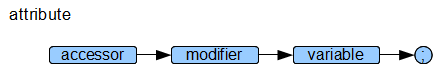
\includegraphics{capitulo09/attribute.png}
 \caption{Atributos}
\end{figure}
% ---------------------------
\subsection{accessor}

\begin{lstlisting}
accessor

   public
   private
   protected
   "default"

\end{lstlisting}

\begin{figure}[h!]
 \centering
 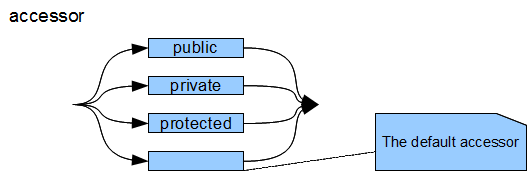
\includegraphics{capitulo09/accessor.png}
 \caption{Acessores}
\end{figure}
% ---------------------------
\subsection{modifier}

\begin{lstlisting}
modifier

   modifier
   modifier modifier
   static
   final

\end{lstlisting}

\begin{figure}[h!]
 \centering
 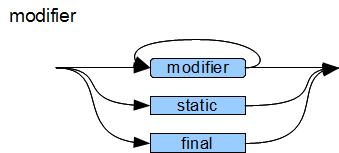
\includegraphics{capitulo09/modifier.png}
 \caption{Modificadores}
\end{figure}
% ---------------------------
\subsection{variable}

\begin{lstlisting}
variable

   type typeName

\end{lstlisting}

\begin{figure}[h!]
 \centering
 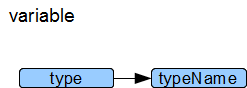
\includegraphics{capitulo09/variable.png}
 \caption{Variável}
\end{figure}
% ---------------------------
\subsection{type}

\begin{lstlisting}
type

   ClassName
   Collection
   primitive

\end{lstlisting}

\begin{figure}[h!]
 \centering
 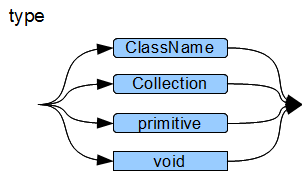
\includegraphics{capitulo09/type.png}
 \caption{Declaração do tipo}
\end{figure}
% ---------------------------
\subsection{primitive}

\begin{lstlisting}
primitive

   byte
   short
   int
   long
   float
   double
   boolean
   char

\end{lstlisting}

\begin{figure}[h!]
 \centering
 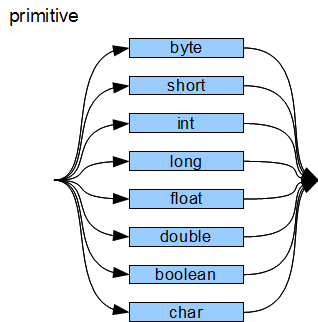
\includegraphics[scale=0.8]{capitulo09/primitive.png}
 \caption{Tipos primitivos}
\end{figure}
% ---------------------------
\subsection{typeName}

\begin{lstlisting}
typeName

   ([a-z0-9][A-Z]+){2,}

\end{lstlisting}

\begin{figure}[h!]
 \centering
 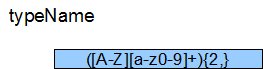
\includegraphics{capitulo09/typeName.png}
 \caption{Nome do tipo}
\end{figure}
% ---------------------------
\subsection{Collection}

\begin{lstlisting}
Collection

   CollectionName < ClassName >

\end{lstlisting}

\begin{figure}[h!]
 \centering
 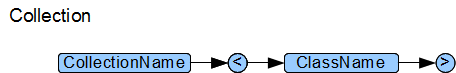
\includegraphics{capitulo09/Collection.png}
 \caption{Definição de coleção}
\end{figure}
% ---------------------------
\subsection{CollectionName}

\begin{lstlisting}
CollectionName

   List
   Set
   Map

\end{lstlisting}

\begin{figure}[h!]
 \centering
 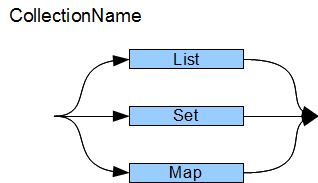
\includegraphics[scale=0.7]{capitulo09/CollectionName.png}
 \caption{Nome da coleção}
\end{figure}
% ---------------------------
\subsection{method}

\begin{lstlisting}
method

   accessor modifier methodIdentifier ( ) { body }
   accessor modifier methodIdentifier ( paramList ) { body }

\end{lstlisting}

\begin{figure}[h!]
 \centering
 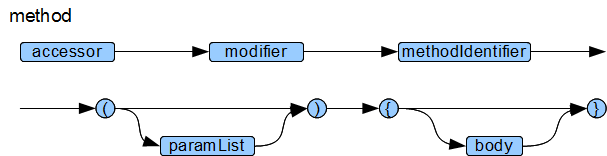
\includegraphics[scale=0.7]{capitulo09/method.png}
 \caption{Definição do método}
\end{figure}
% ---------------------------
\subsection{methodIdentifier}

\begin{lstlisting}
methodIdentifier

   type methodName

\end{lstlisting}

\begin{figure}[h!]
 \centering
 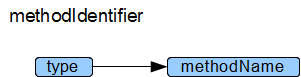
\includegraphics{capitulo09/methodIdentifier.png}
 \caption{Identificação do método}
\end{figure}
% ---------------------------
\subsection{methodName}

\begin{lstlisting}
methodName

   ([a-z0-9][A-Z]+){2,}

\end{lstlisting}

\begin{figure}[h!]
 \centering
 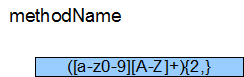
\includegraphics{capitulo09/methodName.png}
 \caption{Nome do método}
\end{figure}
% ---------------------------
\subsection{paramList}

\begin{lstlisting}
paramList

   variable
   variable ,

\end{lstlisting}

\begin{figure}[h!]
 \centering
 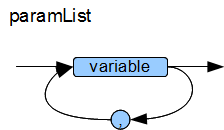
\includegraphics{capitulo09/paramList.png}
 \caption{Lista de parâmetros}
\end{figure}
% ---------------------------
\subsection{body}

\begin{lstlisting}
body

   ""
   statement

\end{lstlisting}

\begin{figure}[h!]
 \centering
 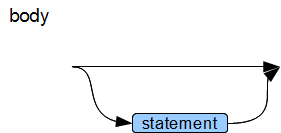
\includegraphics{capitulo09/body.png}
 \caption{Corpo do método}
\end{figure}
% ---------------------------
\subsection{statement}

\begin{lstlisting}
statement

   objectCreation ;
   operationCall ;
   returnStatement ;

\end{lstlisting}

\begin{figure}[h!]
 \centering
 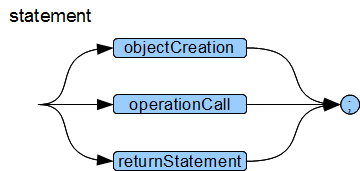
\includegraphics{capitulo09/statement.png}
 \caption{Comandos do método}
\end{figure}
% ---------------------------
\subsection{objectCreation}

\begin{lstlisting}
objectCreation

   ClassName typeName = new ClassName ( )
   ClassName typeName = new ClassName ( paramList )

\end{lstlisting}

\begin{figure}[h!]
 \centering
 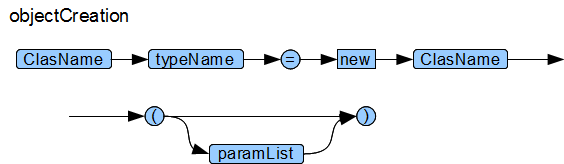
\includegraphics{capitulo09/objectCreation.png}
 \caption{Criação de um objeto}
\end{figure}
% ---------------------------
\newpage
\subsection{operationCall}

\begin{lstlisting}
operationCall

	typeName . methodName ( )
	typeName . methodName ( variableValue )
	typeName . methodName ( variableValue , )

\end{lstlisting}

\begin{figure}[h!]
 \centering
 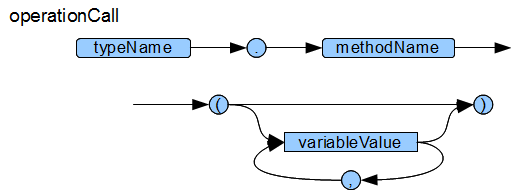
\includegraphics{capitulo09/operationCall.png}
 \caption{Chamada de um métodos}
\end{figure}
% ---------------------------
\subsection{returnStatement}

\begin{lstlisting}
returnStatement

    return type

\end{lstlisting}

\begin{figure}[h!]
 \centering
 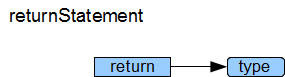
\includegraphics{capitulo09/returnStatement.png}
 \caption{Comando de retorno}
\end{figure}

\end{document}

% Fim do documento